\documentclass[tikz,border=5mm]{standalone}

\begin{document}

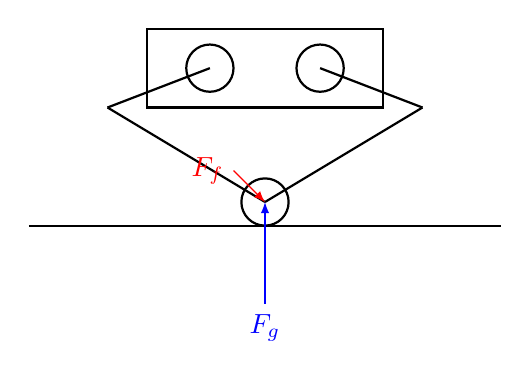
\begin{tikzpicture}[>=latex]

% Draw the ground
\draw[thick] (-3,0) -- (3,0);

% Draw the body
\draw[thick] (-1.5,1.5) rectangle (1.5,2.5);

%% Draw the wheel
\draw[thick] (-0.7,2) circle (0.3);
\draw[thick] (0.7,2) circle (0.3);
\draw[thick] (-0.7,2) -- (-2,1.5);
\draw[thick] (0.7,2) -- (2,1.5);
\draw[thick] (2,1.5) -- (0,0.3);
\draw[thick] (-2,1.5) -- (0,0.3);
\draw[thick] (0,0.3) circle (0.3);

%% Add gravity and friction
\draw[<-,blue] (0,0.3) -- (0,-1) node[below] {$F_g$};
\draw[<-,red] (0,0.3) -- (-0.4,0.7) node[left] {$F_f$};

\end{tikzpicture}

\end{document}